%\gls{UML}........\acrshort{UML}
\chapter{Requirements analysis}
\newpage
\section*{Introduction}
In this chapter, we will cover the project requirements, prototypes, the modeling and design.
\addcontentsline{toc}{section}{Introduction}
\section{Requirements analysis}

\subsection{Use case diagram}

\begin{figure}[!ht]
    \centering
    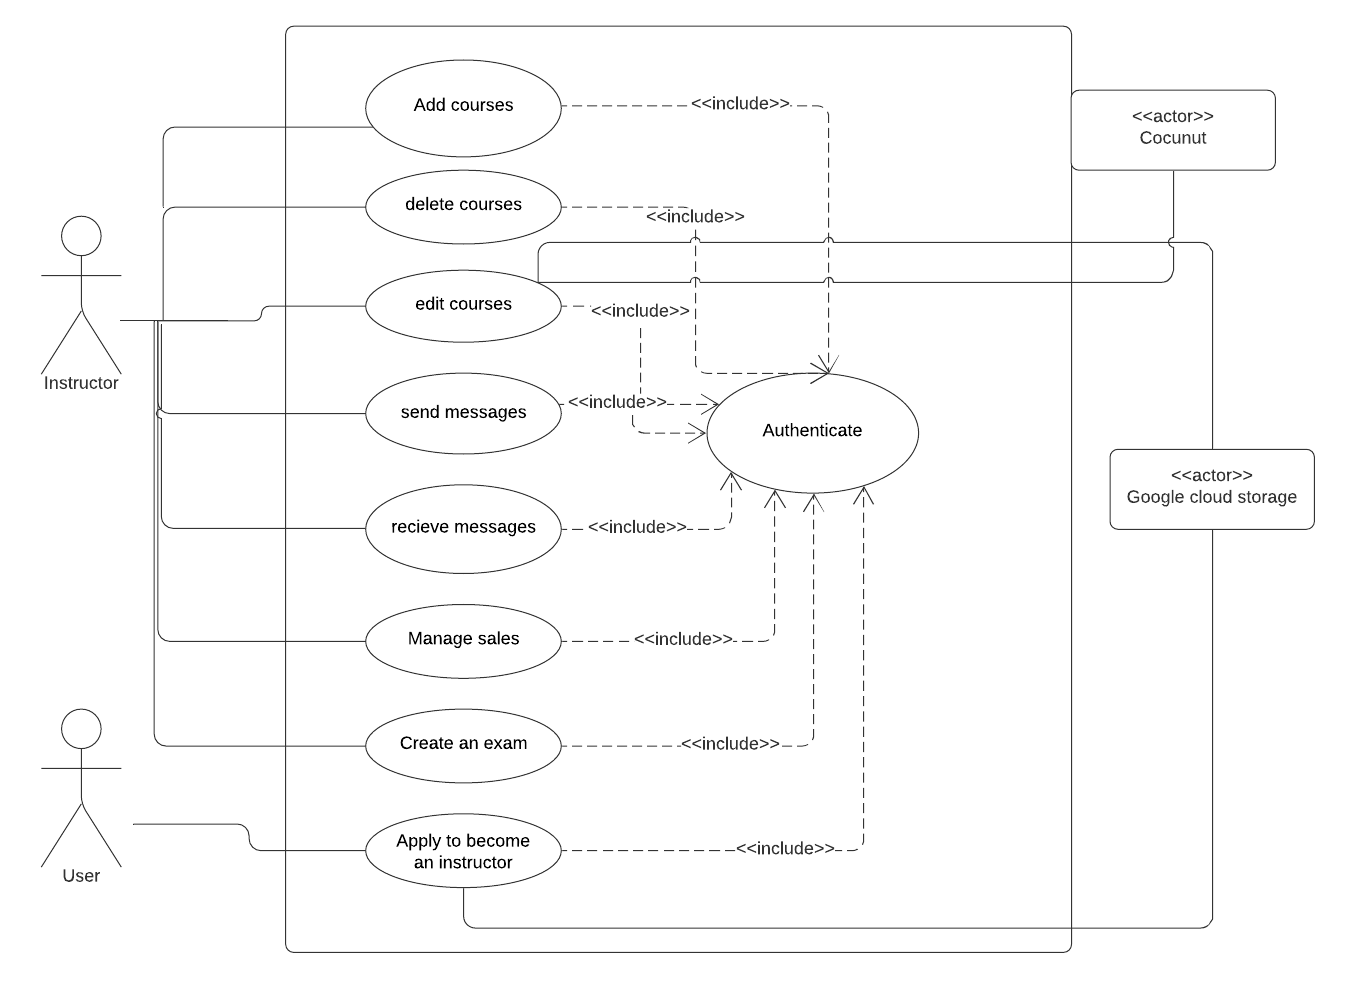
\includegraphics[width=170mm]{use_case.png}
    \caption{Use case diagram}
    \label{fig:use_case}
\end{figure}


\subsection{Use case diagram details}
\hfill \break
\textbf{Coconut :} coconut is the transcoding service that we use to transcode the videos uploaded (Build multiple resolution streamable video versions).
\hfill \break
\textbf{Google cloud storage :} is the service where we store the uploaded files and course videos.
\hfill \break
\textbf{Instructor :} is the user of the instructor dashboard.
\hfill \break
\textbf{User :} is a normal user that is not an instructor.
 

\subsection{Database schema}

The figure below shows the database schema that is already built.

\begin{figure}[!ht]
    \centering
    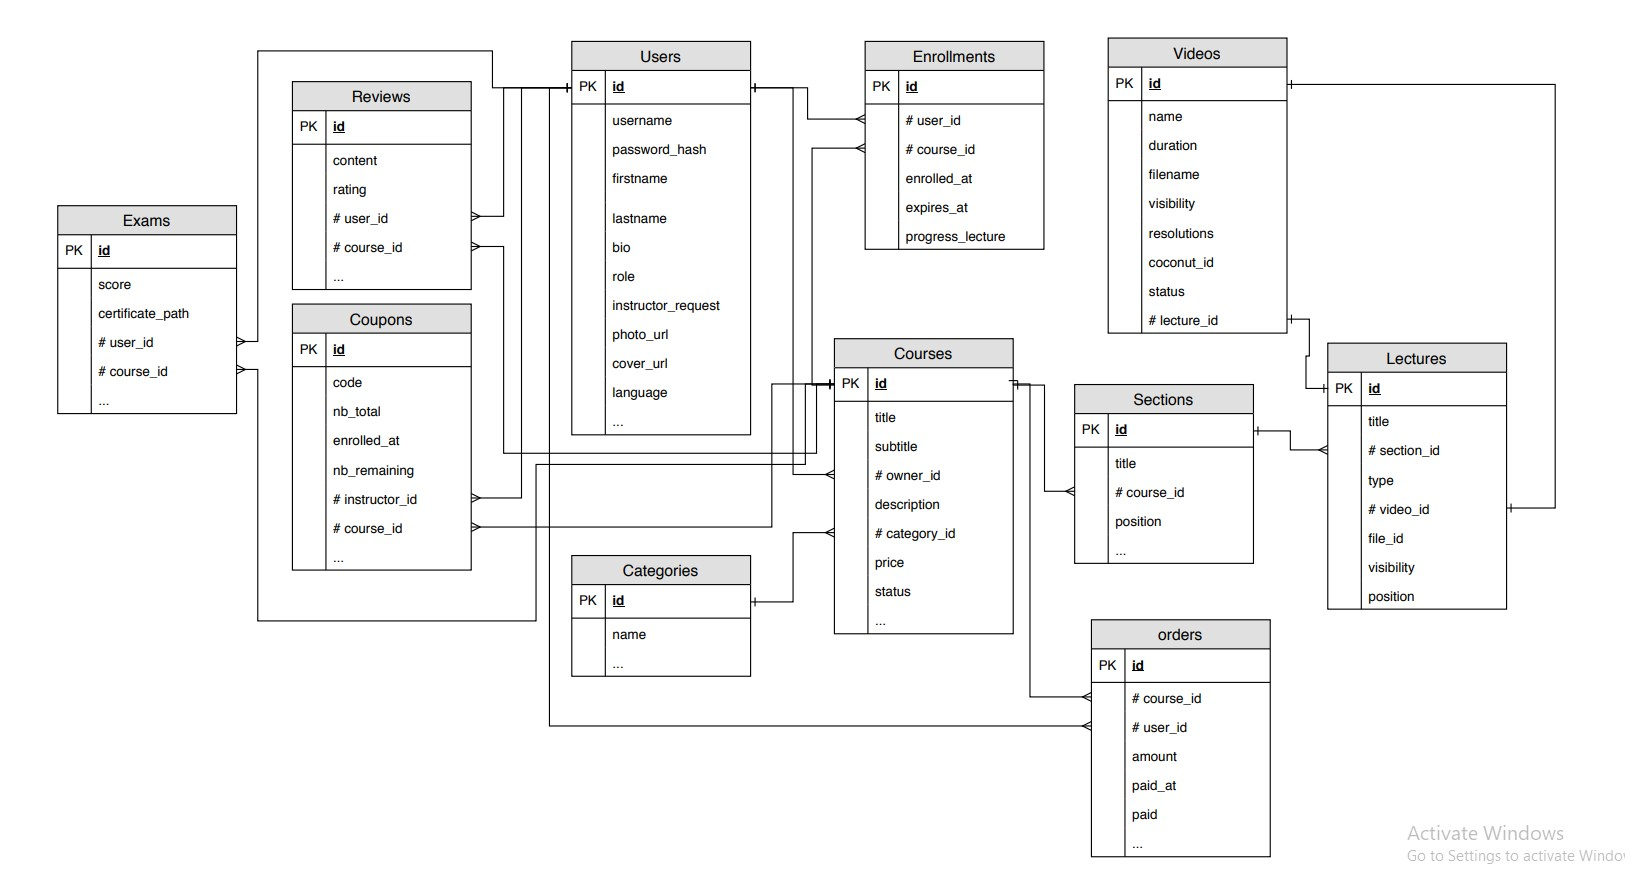
\includegraphics[width=170mm]{database_schema.jpg}
    \caption{Database schema}
    \label{fig:database_schema}
\end{figure}


\subsection{Functional requirements}
\begin{itemize}
    \item[\ding{81}] Instructor must be able to add courses.
    \item[\ding{81}] Instructor must be able to delete courses.
    \item[\ding{81}] Instructor must be able to edit courses.
    \item[\ding{81}] Instructor must be able to send messages to students.
    \item[\ding{81}] Instructor must be able to recieve messages from students.
    \item[\ding{81}] Instructor must be able to see courses sales.
    \item[\ding{81}] Instructor must be able to create an exam.
    \item[\ding{81}] User must be able to apply to become an instructor.
\end{itemize}
\subsection{Non functional requirements}
\begin{itemize}
    \item[\ding{81}] The application must be efficient and have low response time.
    \item[\ding{81}] The application must be secure.
    \item[\ding{81}] The application must be simple to use. The user must not encounter any obstacles or ambiguity during his experience.
\end{itemize}

\section{Prototypes}
This section will show the wireframes created using Adobe XD.

\subsection{Courses tab}

The figure below shows the courses tab where the instructor can see his courses.

\begin{figure}[!ht]
    \centering
    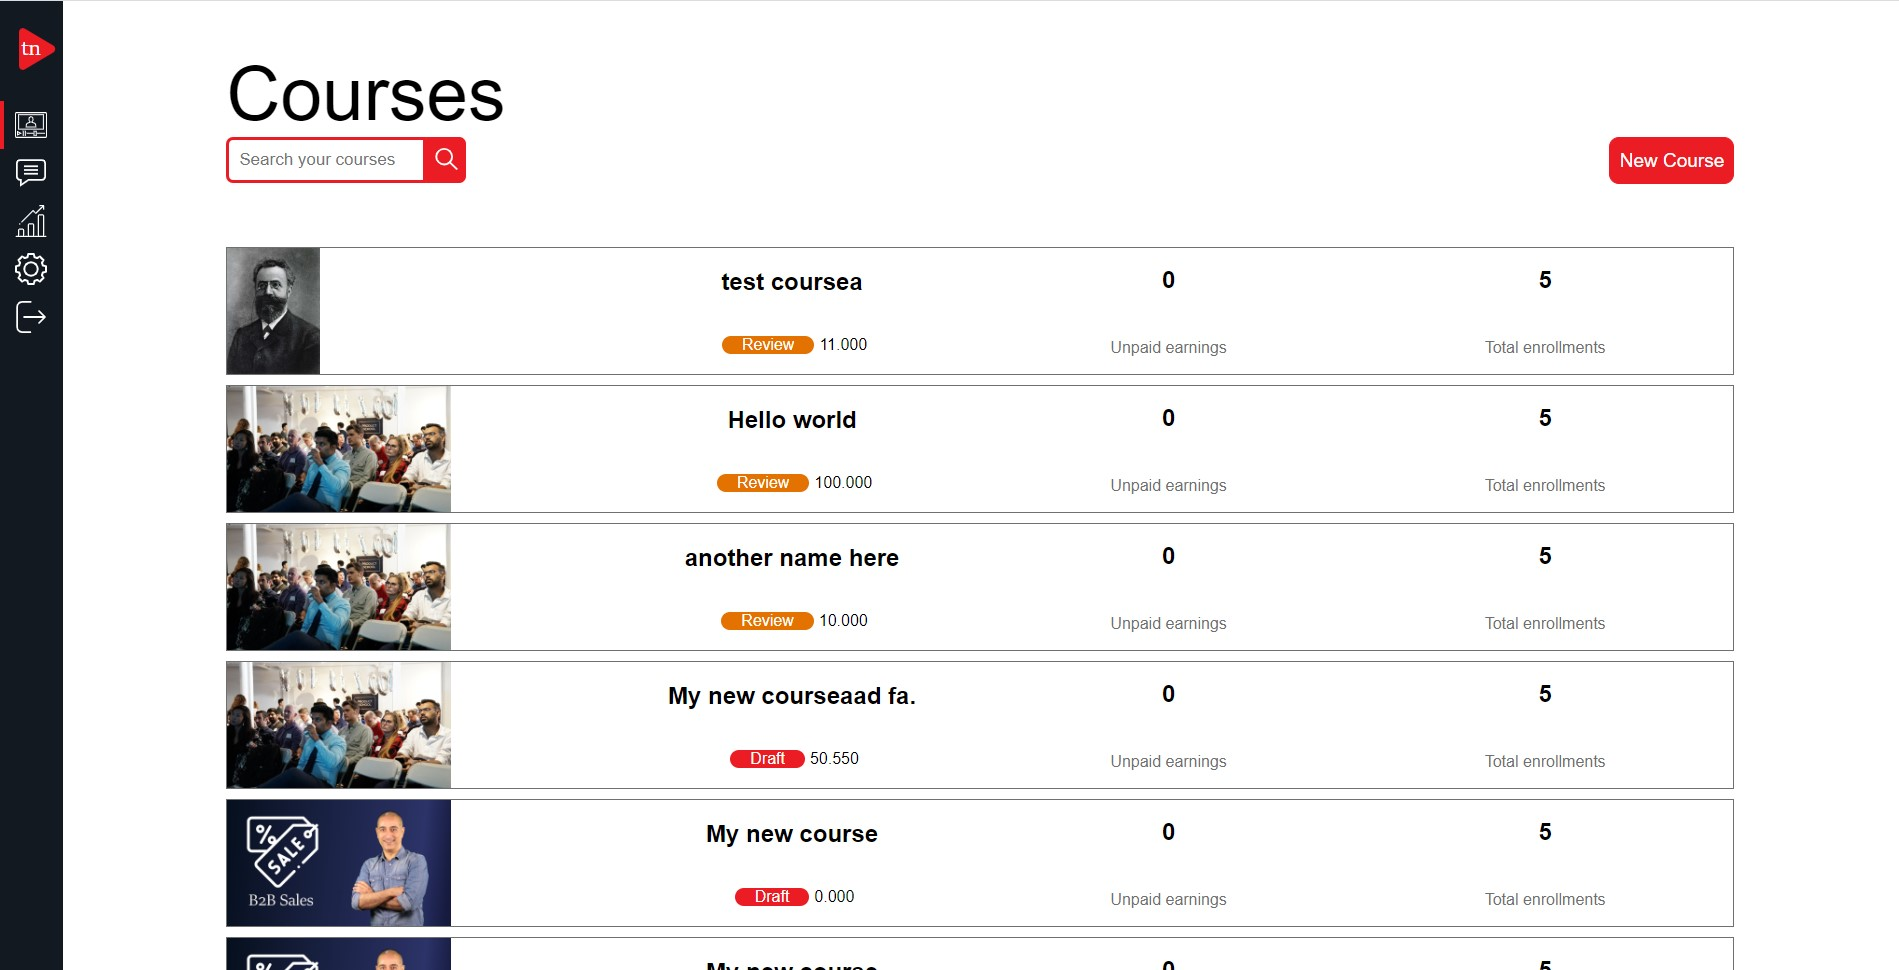
\includegraphics[width=170mm]{courses_tab.jpg}
    \caption{Wireframe for the courses tab}
    \label{fig:courses_tab}
\end{figure}


\vfill
\clearpage

\subsection{Edit course}


The figure below shows the curriculum form where the instructor can add chapters, lectures, and attaches videos to them.

\begin{figure}[!ht]
    \centering
    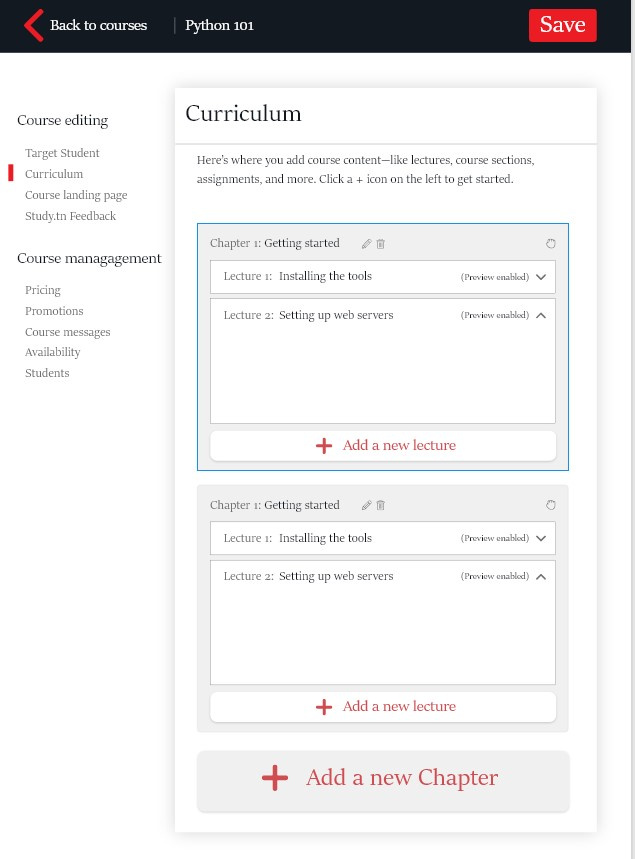
\includegraphics[width=150mm]{edit_course_cir_form.jpg}
    \caption{Wireframe for the curriculum form}
    \label{fig:edit_course_cir_form}
\end{figure}

The figure below shows the landing page form where the instructor can edit the course data like title, and description.

\begin{figure}[!ht]
    \centering
    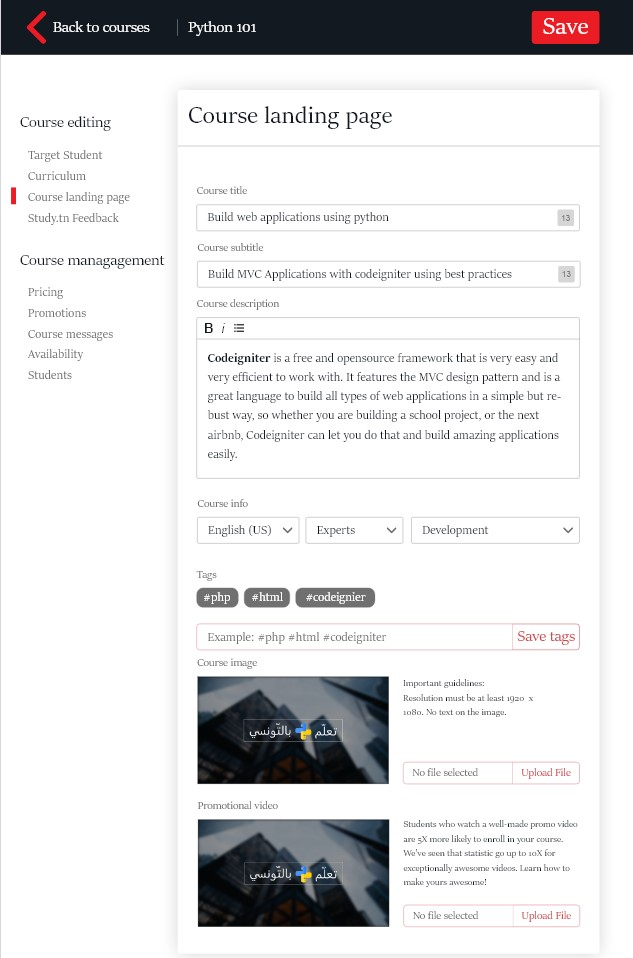
\includegraphics[width=150mm]{edit_course_landing_page_form.jpg}
    \caption{Wireframe for the landing page form}
    \label{fig:edit_course_landing_page_form}
\end{figure}

The figure below shows the pricing form where the instructor can edit his course price.

\begin{figure}[!ht]
    \centering
    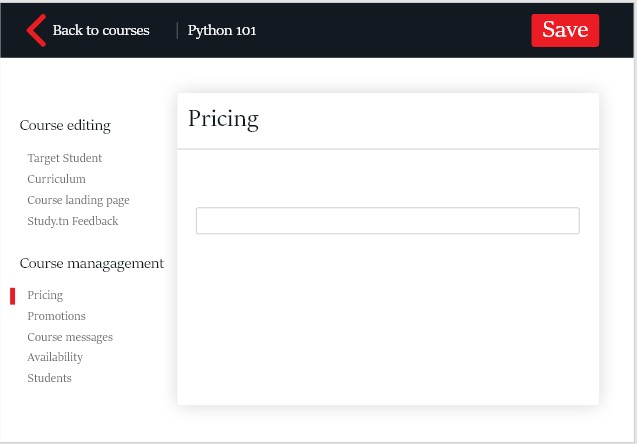
\includegraphics[width=150mm]{edit_course_price.jpg}
    \caption{Wireframe for the price form}
    \label{fig:edit_course_price}
\end{figure}

\vfill
\clearpage

The figure below shows the target students form where the instructor can define the requirements needed before taking the course.

\begin{figure}[!ht]
    \centering
    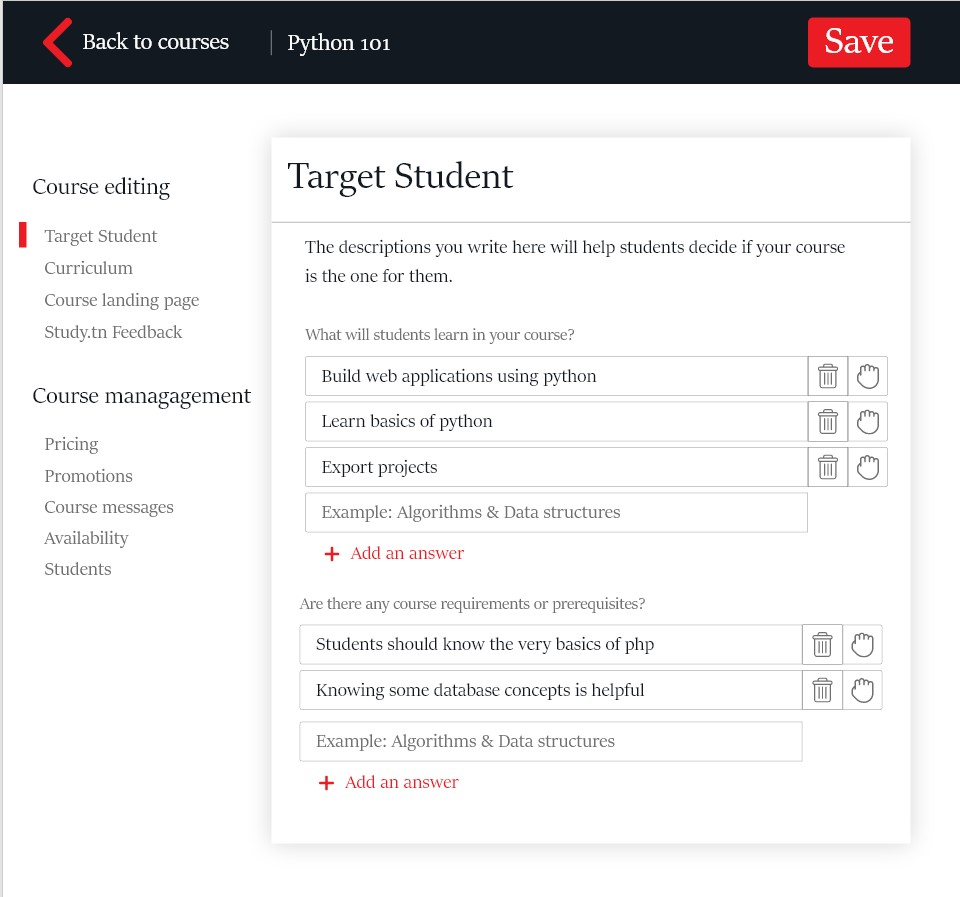
\includegraphics[width=150mm]{edit_course_target_form.jpg}
    \caption{Wireframe for the target students form}
    \label{fig:edit_course_target_form}
\end{figure}

\vfill
\clearpage

\subsection{Communication}

The figures below show the communication part of the dashboard.

\begin{figure}[!ht]
    \centering
    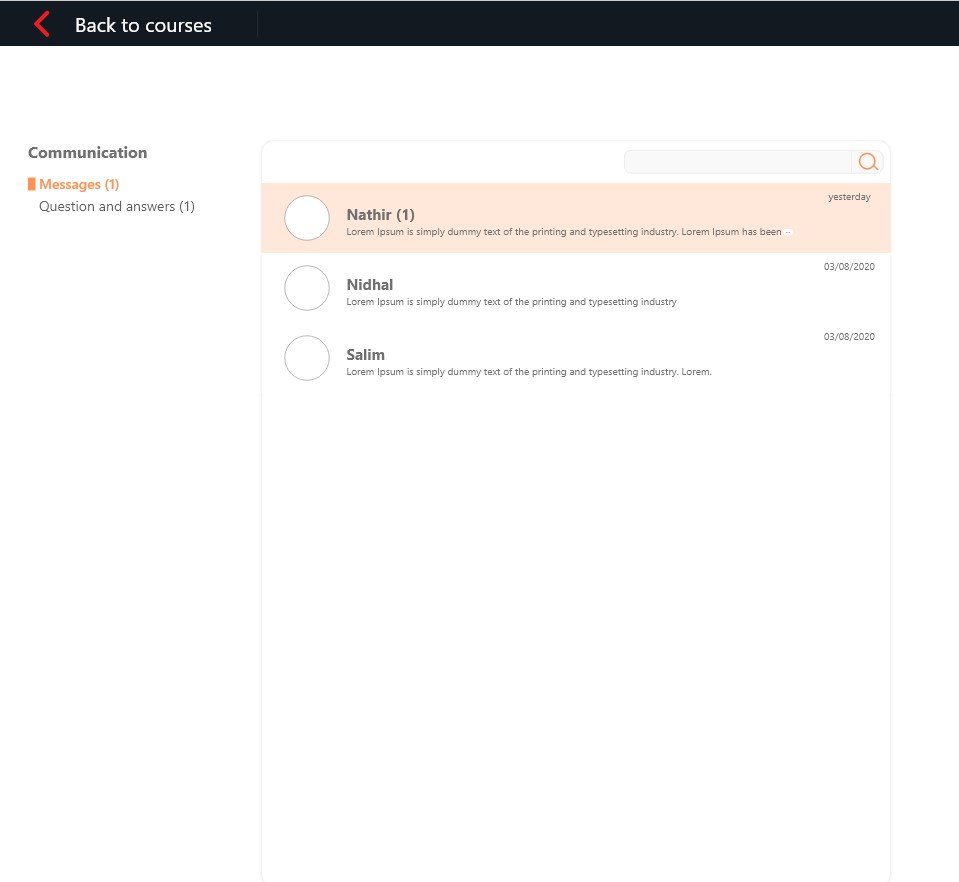
\includegraphics[width=150mm]{conversation_list.jpg}
    \caption{Wireframe for the conversations list}
    \label{fig:conversation_list}
\end{figure}


\vfill
\clearpage

\begin{figure}[!ht]
    \centering
    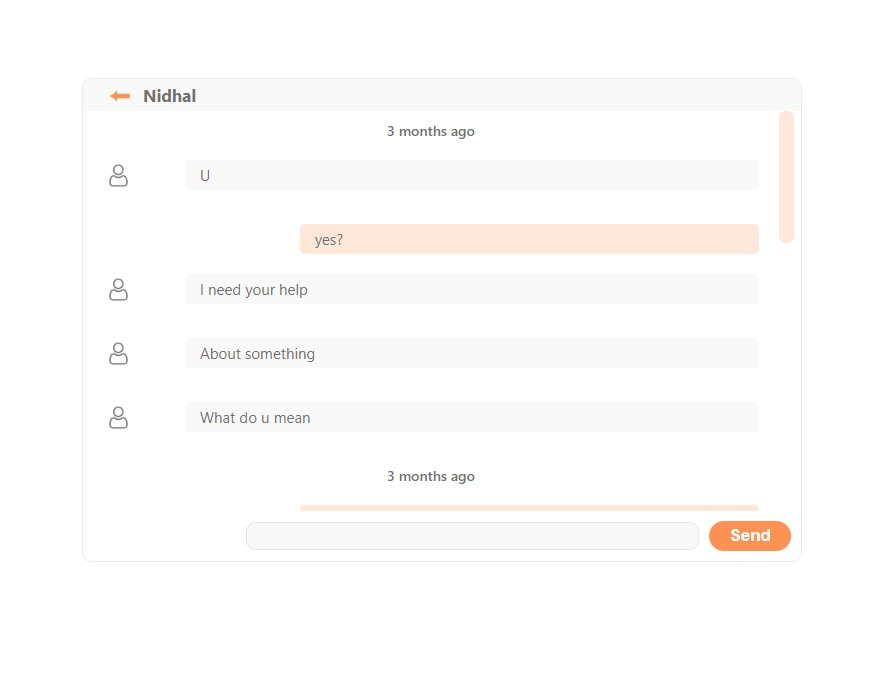
\includegraphics[width=170mm]{conversation.jpg}
    \caption{Wireframe for a conversation}
    \label{fig:conversation}
\end{figure}


\section{Modeling and approach}

\subsection{Product backlog}
%%%%%table
\begin{table}[H]
\centering
\caption{Product backlog}
\begin{tabular}{|p{1cm}|p{1.5cm}|p{3cm}|p{6cm}|p{2cm}|}
\hline
\rowcolor{brown!18}\textbf{\large{ID}} & \textbf{\large{Sprint}} & \textbf{\large{As a}}  & \textbf{\large{I want to be able to}} & \textbf{\large{Priority}} \\
\hline
1& 1 & Instructor & Access the instructor space & High\\\hline
2& 1 & Instructor & Add courses  & High\\\hline
3& 1 & Instructor & Delete my courses  & High\\\hline
4& 1& Instructor & Edit my courses  & High\\\hline
5& 2& Instructor & Send messages to my students & High\\\hline
6& 2& Instructor & Recieve messages from my students  & High\\\hline
7& 2& Instructor  & See my course sales & Normal \\\hline
8& 3& Instructor & Create an exam & High\\\hline
9& 3& User & Apply to become an instuctor  & Normal \\\hline
\end{tabular}
\end{table}


\subsection{Use case diagram for each sprint}

\begin{figure}[!ht]
\centering
     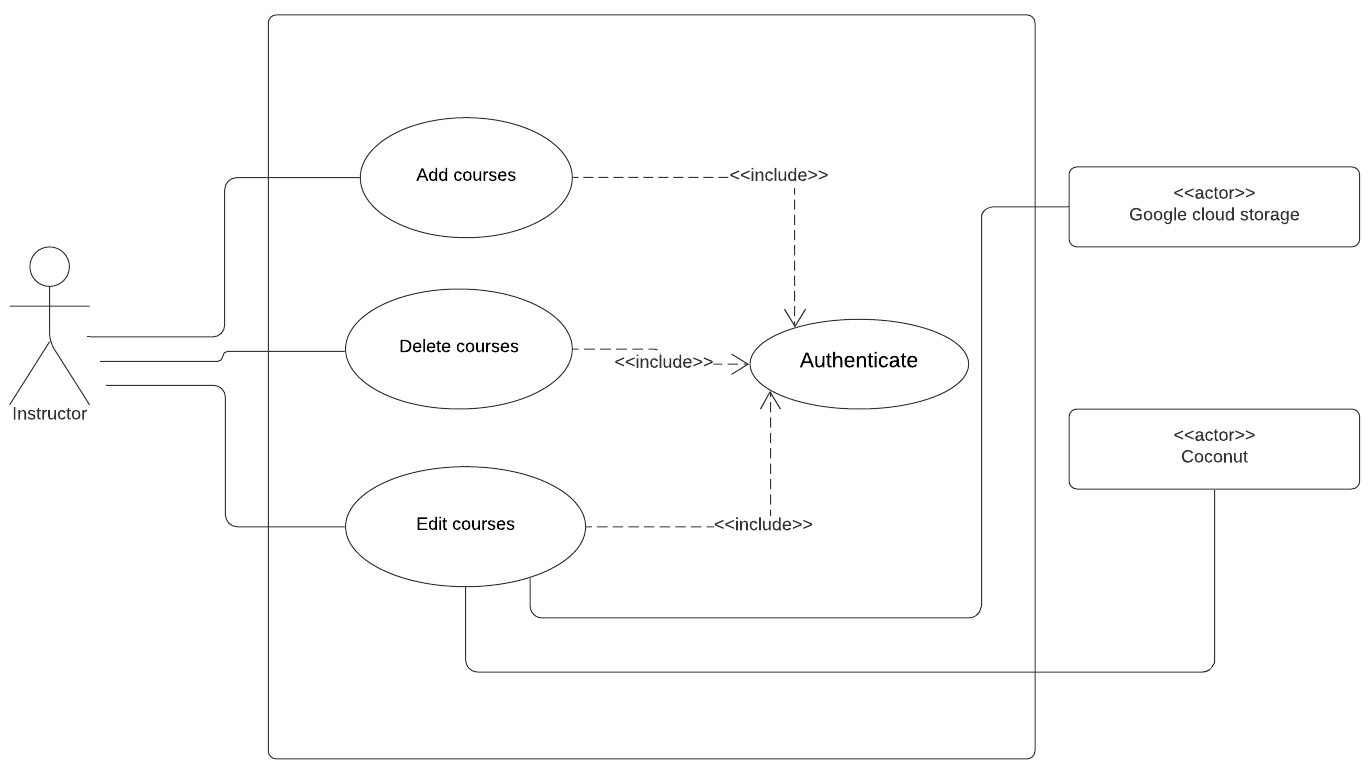
\includegraphics[width=150mm]{sprint1usecase.png}
    \caption{Sprint 1 use case diagram}
    \label{fig:sprint1usecase}
\end{figure}

\begin{figure}[!ht]
    \centering
    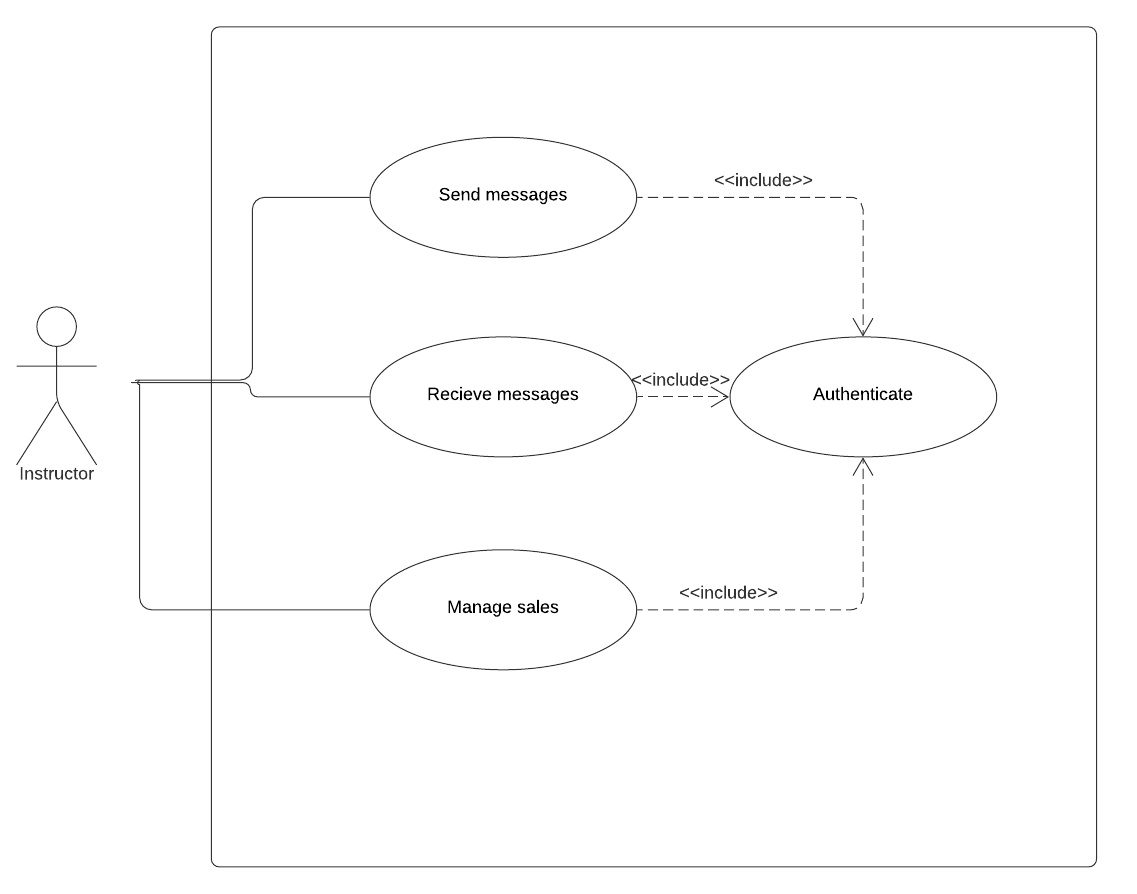
\includegraphics[width=120mm]{sprint2usecase.png}
    \caption{Sprint 2 use case diagram}
    \label{fig:sprint2usecase}
\end{figure}


\begin{figure}[!ht]
    \centering
    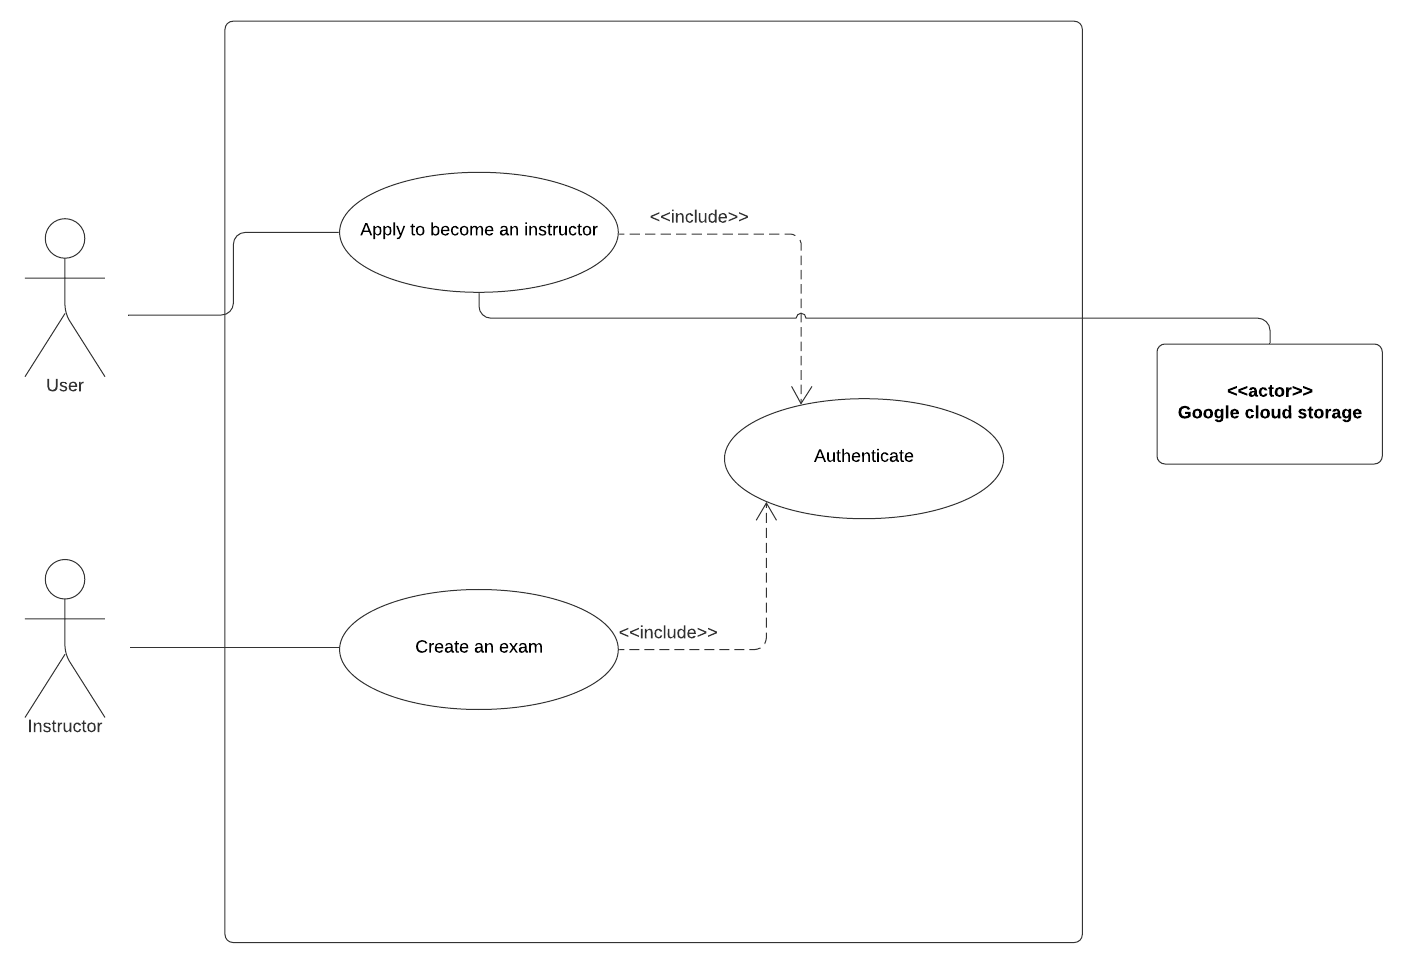
\includegraphics[width=125mm]{sprint3usecase.png}
    \caption{Sprint 3 use case diagram}
    \label{fig:sprint3usecase}
\end{figure}

\section*{Conclusion}
This chapter is important and crucial to ensure efficiency during the project implementation. We first identified the actors and needs, which allowed us to break down the project into functionalities and tasks. Then we planned the tasks according to the Scum methodology that was chosen.
